\documentclass[12pt]{article}
\usepackage[utf8]{inputenc}
\usepackage[T1]{fontenc}
\usepackage[a4paper]{geometry}
\geometry{hscale=0.80,vscale=0.80,centering}
\usepackage{amsmath}
\usepackage{amsthm}
\usepackage{stmaryrd}
\usepackage{amssymb}
\usepackage{breqn}
\usepackage{graphicx}
\usepackage[affil-it]{authblk}
\newcommand{\Mod}[1]{\ (\mathrm{mod}\ #1)}
\title{Projet P-A.N.D.R.O.I.D.E.\\
\bigbreak\textbf{Branch and Bound pour les diagrammes d'influence}}
\author{PINAUD David \& BIEGAS Emilie}
\date{Janvier 2021}
\affil{Université Sorbonne Sciences}
\begin{document}
\maketitle

\renewcommand{\contentsname}{Table des Matières}
\pagebreak
\tableofcontents
\pagebreak

\section{Introduction}

\subsection{Les diagrammes d'influence (ID)}
Les diagrammes d'influence (ID) sont des graphes acycliques dirigés présentant trois types de nœuds. Les nœuds de \textit{chance}, illustrés graphiquement par un ovale, représentent des variables aléatoire (dont le domaine est fini et non vide). 
Les nœuds de \textit{décision}, illustrés graphiquement par un rectangle, représentent des variables de décision (dont le domaine est fini et non vide) tandis que les nœuds d'\textit{utilité}, illustrés graphiquement par un losange, représentent une fonction d'utilité locale exprimant la préférence.
Lorsqu'il y a plusieurs nœuds d'utilité, l'utilité totale en est la somme (c'est une décomposition partiellement additive de l'utilité).
\bigbreak
Les arcs de ce graphe représentent une dépendance entre les nœuds et ont une signification différente en fonction du type de nœud à son extrémité.
En effet, si un arc pointe vers un nœud de chance, cela représente une dépendance probabiliste; si il pointe vers un nœud de décision, il a un but informatif; enfin, si il pointe vers un nœud d'utilité, il représente une dépendance fonctionnelle.
\bigbreak
Les IDs respectent deux hypothèses, une hypothèse de régularité (les décisions sont ordonnées dans le temps) et une hypothèse dite non-oubliant (chaque décision est conditionnée par toutes les observations de décisions antérieures).
L'ensemble des instanciations des nœuds de chance pour les décisions antérieures d'une certaine désicion est appelé l'\textit{historique}.


\subsection{Les LIMIDs}
 Les \textit{LImited-Memory Influence-Diagrams} (LIMIDs) sont des diagrammes d'influence qui assouplissent les deux hypothèses précédemment citées. 
 \bigbreak
 Tout d'abord, les LIMIDs assouplissent l'hypothèse non-oubliant de manière à conditionner une décision sur un nombre limité d'observations et de décisions antérieurs pertinentes (pour un compromis qualité/complexité).
\bigbreak
Ensuite, assouplir l'hypothèse de régularité permet par exemple de modéliser la coopération de problèmes de décision multi-agents où un agent n'est pas au courant de décision d'autres agents. 
Les IDs forment alors un sous-ensemble des LIMIDs.

\subsection{Limites des implémentations actuelles}
Les méthodes de résolution exactes actuelles de LIMIDs ou IDs sont limités par leur complexité en temps et en espace.
Pour exemple, considérons un ID qui modélise un robot dans un labyrinthe représenté par une matrice $n\times m$ composé de cases \textit{mur}, de cases \textit{libre} et d'une case \textit{objectif}. On représente le labyrinthe comme ci-dessous, les cases grises, blanches, et étoilés étant respectivement les cases \textit{mur}, \textit{libre}, et \textit{objectif}.
\begin{figure}[h]
\centering
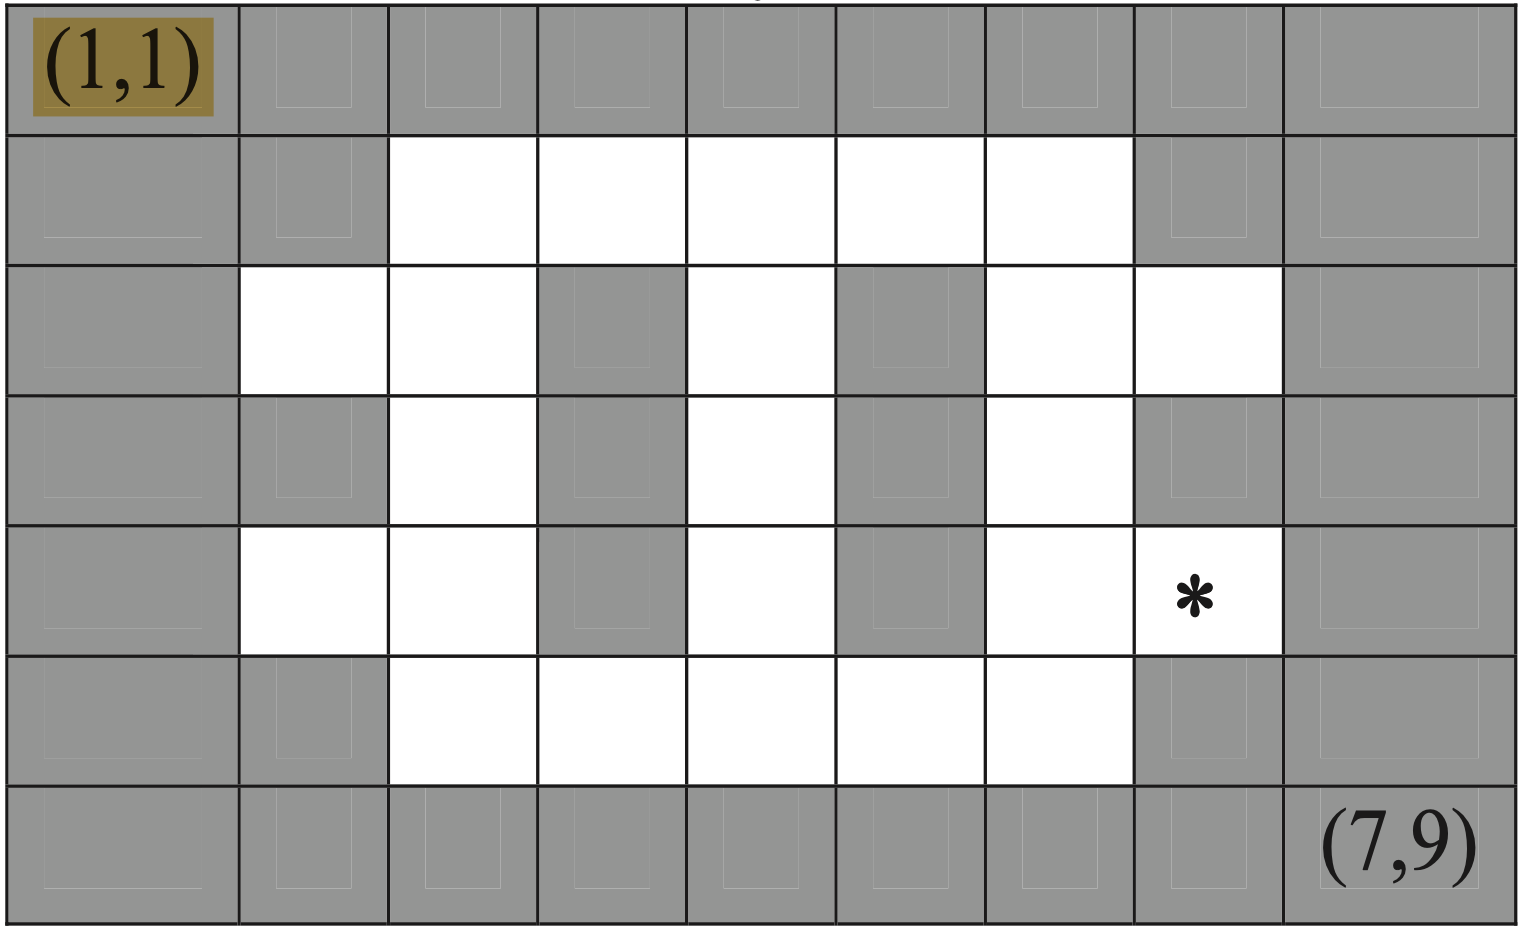
\includegraphics[scale=0.2]{docs/ressources_rapport/MAZE.png}
\caption{Un exemple de représentation d'un labyrinthe $9\times 7$}
\end{figure}
\pagebreak


Le robot est initialement placé sur une des cases \textit{libre} et l'objectif du robot est d'atteindre la case \textit{objectif}. 
À chaque étape, le robot peut se déplacer dans toutes les directions (nord, sud, est, ouest et les diagonales) d'une seule case ou choisir de ne pas se déplacer. Il possède quatre capteurs pointés vers les quatre cardinaux qui indiquent au robot la présence d'un mur ou non.
%les probabilités sommes à 1 --> c'est bien une distribution donc pas de mouvement en diagonale possible ?!

À chaque étape, le robot choisit une direction cardinale où faire un pas puis le mouvement du robot suit une mesure de probabilité :
\begin{itemize}
  \item Un pas vers la case voulu a une probabilité $pBouger$ de réussir.
  \item Échouer de bouger survient avec probabilité $pEchecBouger$.
  \item À chaque étape, il y a une chance que le robot fasse un mouvement erratique:
  \begin{itemize}
        \item Faire un pas vers la droite ou vers la gauche (c'est-à-dire vers l'est ou vers l'ouest si son choix est de se diriger vers le nord), s'il est possible de le faire, survient avec une probabilité de $pCote$ dans chacun des deux cas.
        \item Faire un pas en arrière (c'est-à-dire vers le sud si son choix est de se diriger vers le nord), s'il est possible de le faire, survient avec une probabilité $pArriere$.
        \end{itemize}
  \item Un pas vers un \textit{mur} a une probabilité de 0.
  \item Les autres probabilités sont normalisées afin de former une distribution de probabilité.
\end{itemize}
\begin{figure}[h]
\centering
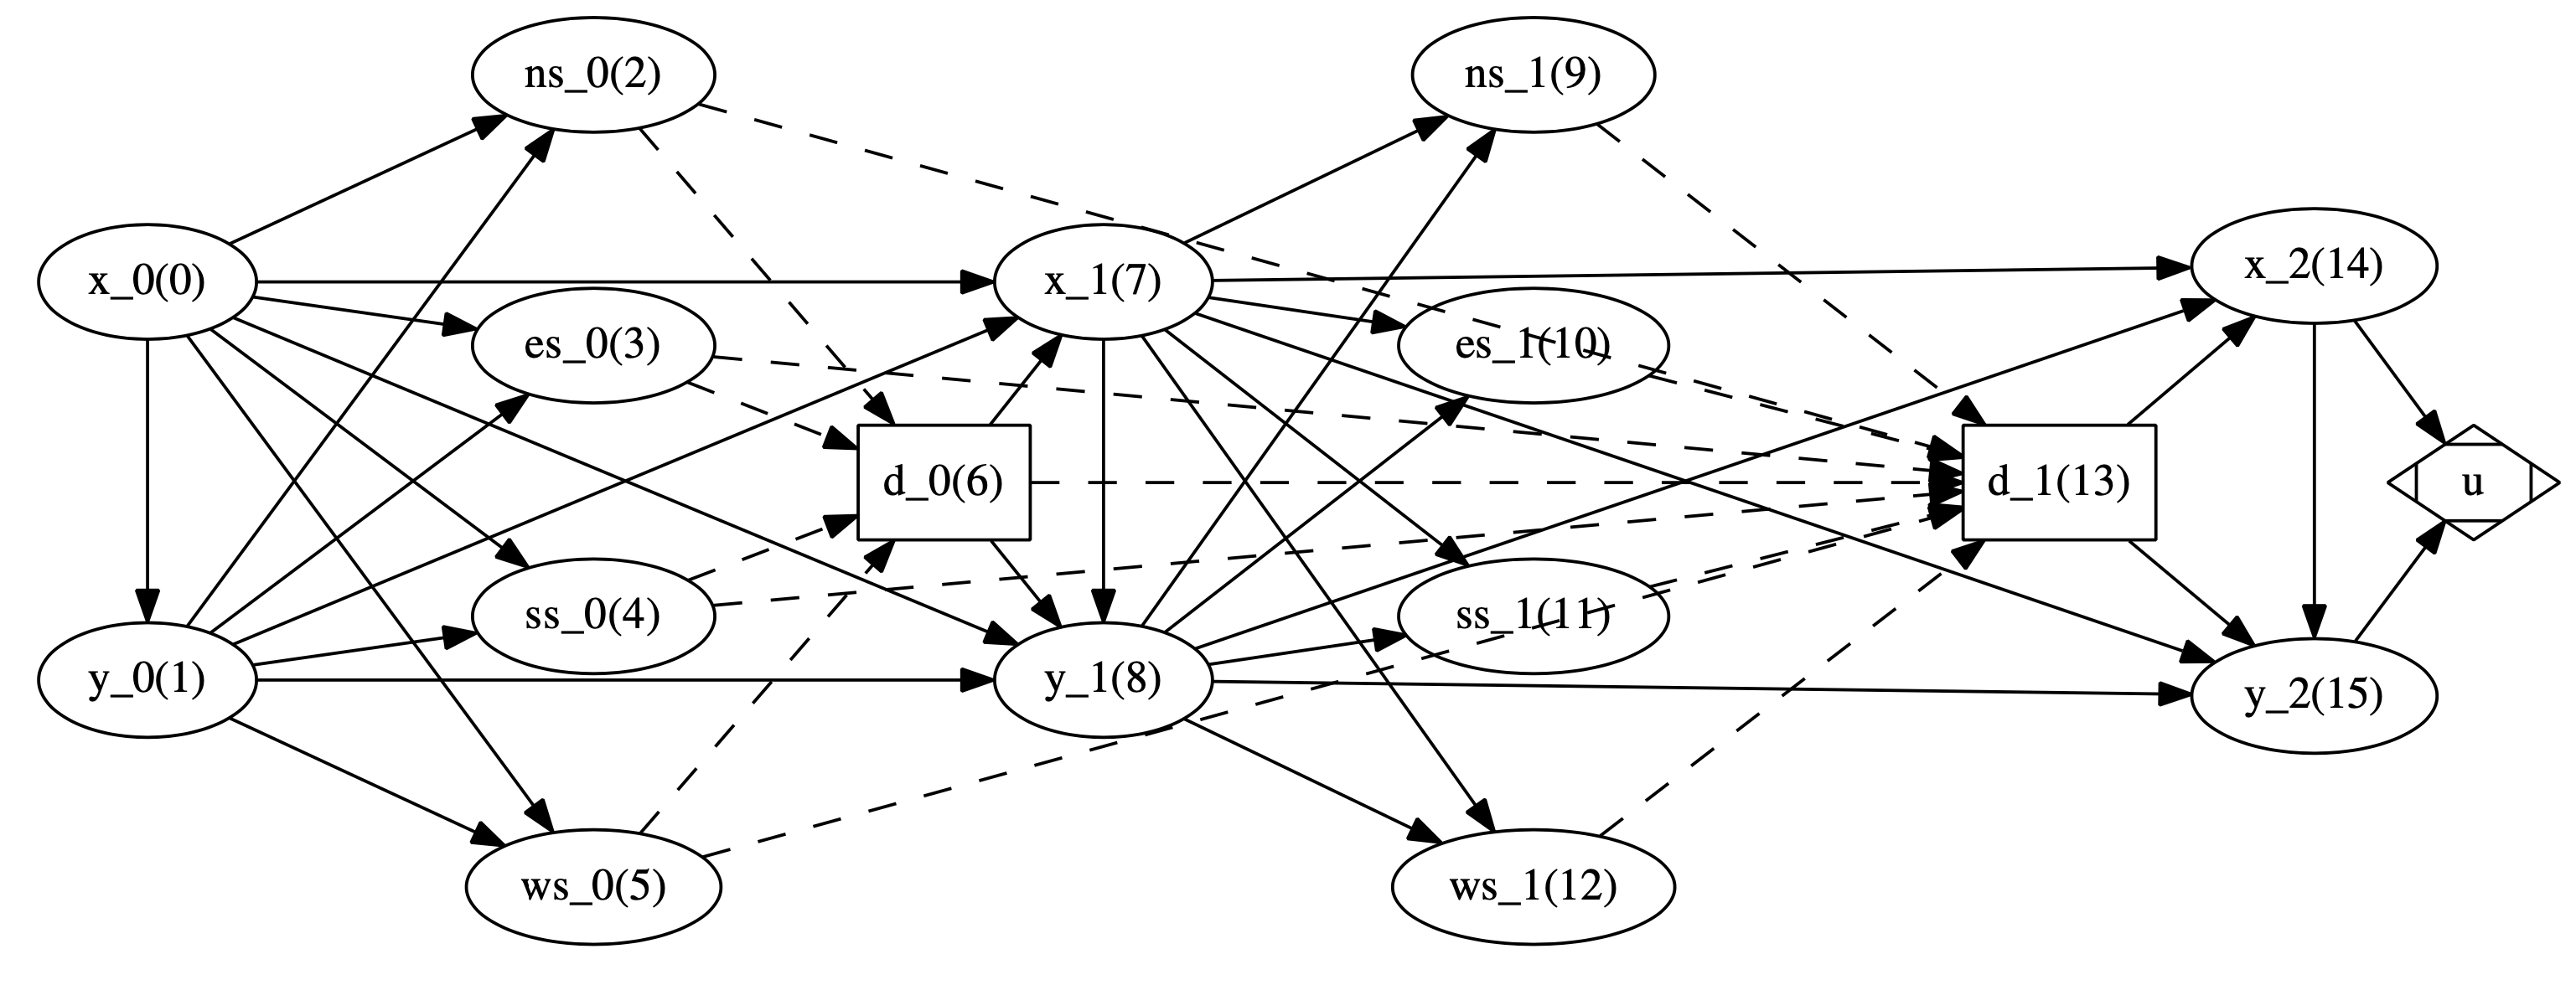
\includegraphics[scale=0.22]{docs/ressources_rapport/IDROBOT.png}
\caption{L'ID modélisant le problème du robot à deux étapes }
\end{figure}
A l'étape $i$, les nœuds de chance $x_i$ et $y_i$ représentent les coordonnées du robot sur la grille, $ns_i, es_i, ss_i, ws_i$ les capteurs du robot dans les sens nord, est, sud et ouest respectivement. Les nœuds $d_i$ sont les nœuds de décision.

\pagebreak
Pour visualiser le caractère exponentiel de la complexité en espace, voici un tableau récapitulatif des tailles des arbres de jonctions selon le nombre d'étapes ainsi que les graphes associés.
\bigbreak
\begin{center}
   \begin{tabular}{|p{3cm} || p{3cm} | p{3cm} | }
    \hline
    Nombre d'étapes & Tree-width (largeur de l'arbre) & taille en mémoire de l'arbre (en Go) \\ 
    \hline
    2&11&2 E-3\\
    \hline
    3&15&38 E-3\\
    \hline
    4&20&787 E-3\\
    \hline
    5&24&12\\
    \hline
    6&29&984\\
    \hline
    7&34&76 E3\\
    \hline
    8&37&246 E3\\
    \hline
    9&42&19687 E3\\
    \hline
    109&46&315000 E3\\
    \hline
   \end{tabular}
\end{center}
 \begin{figure}[h]
\centering
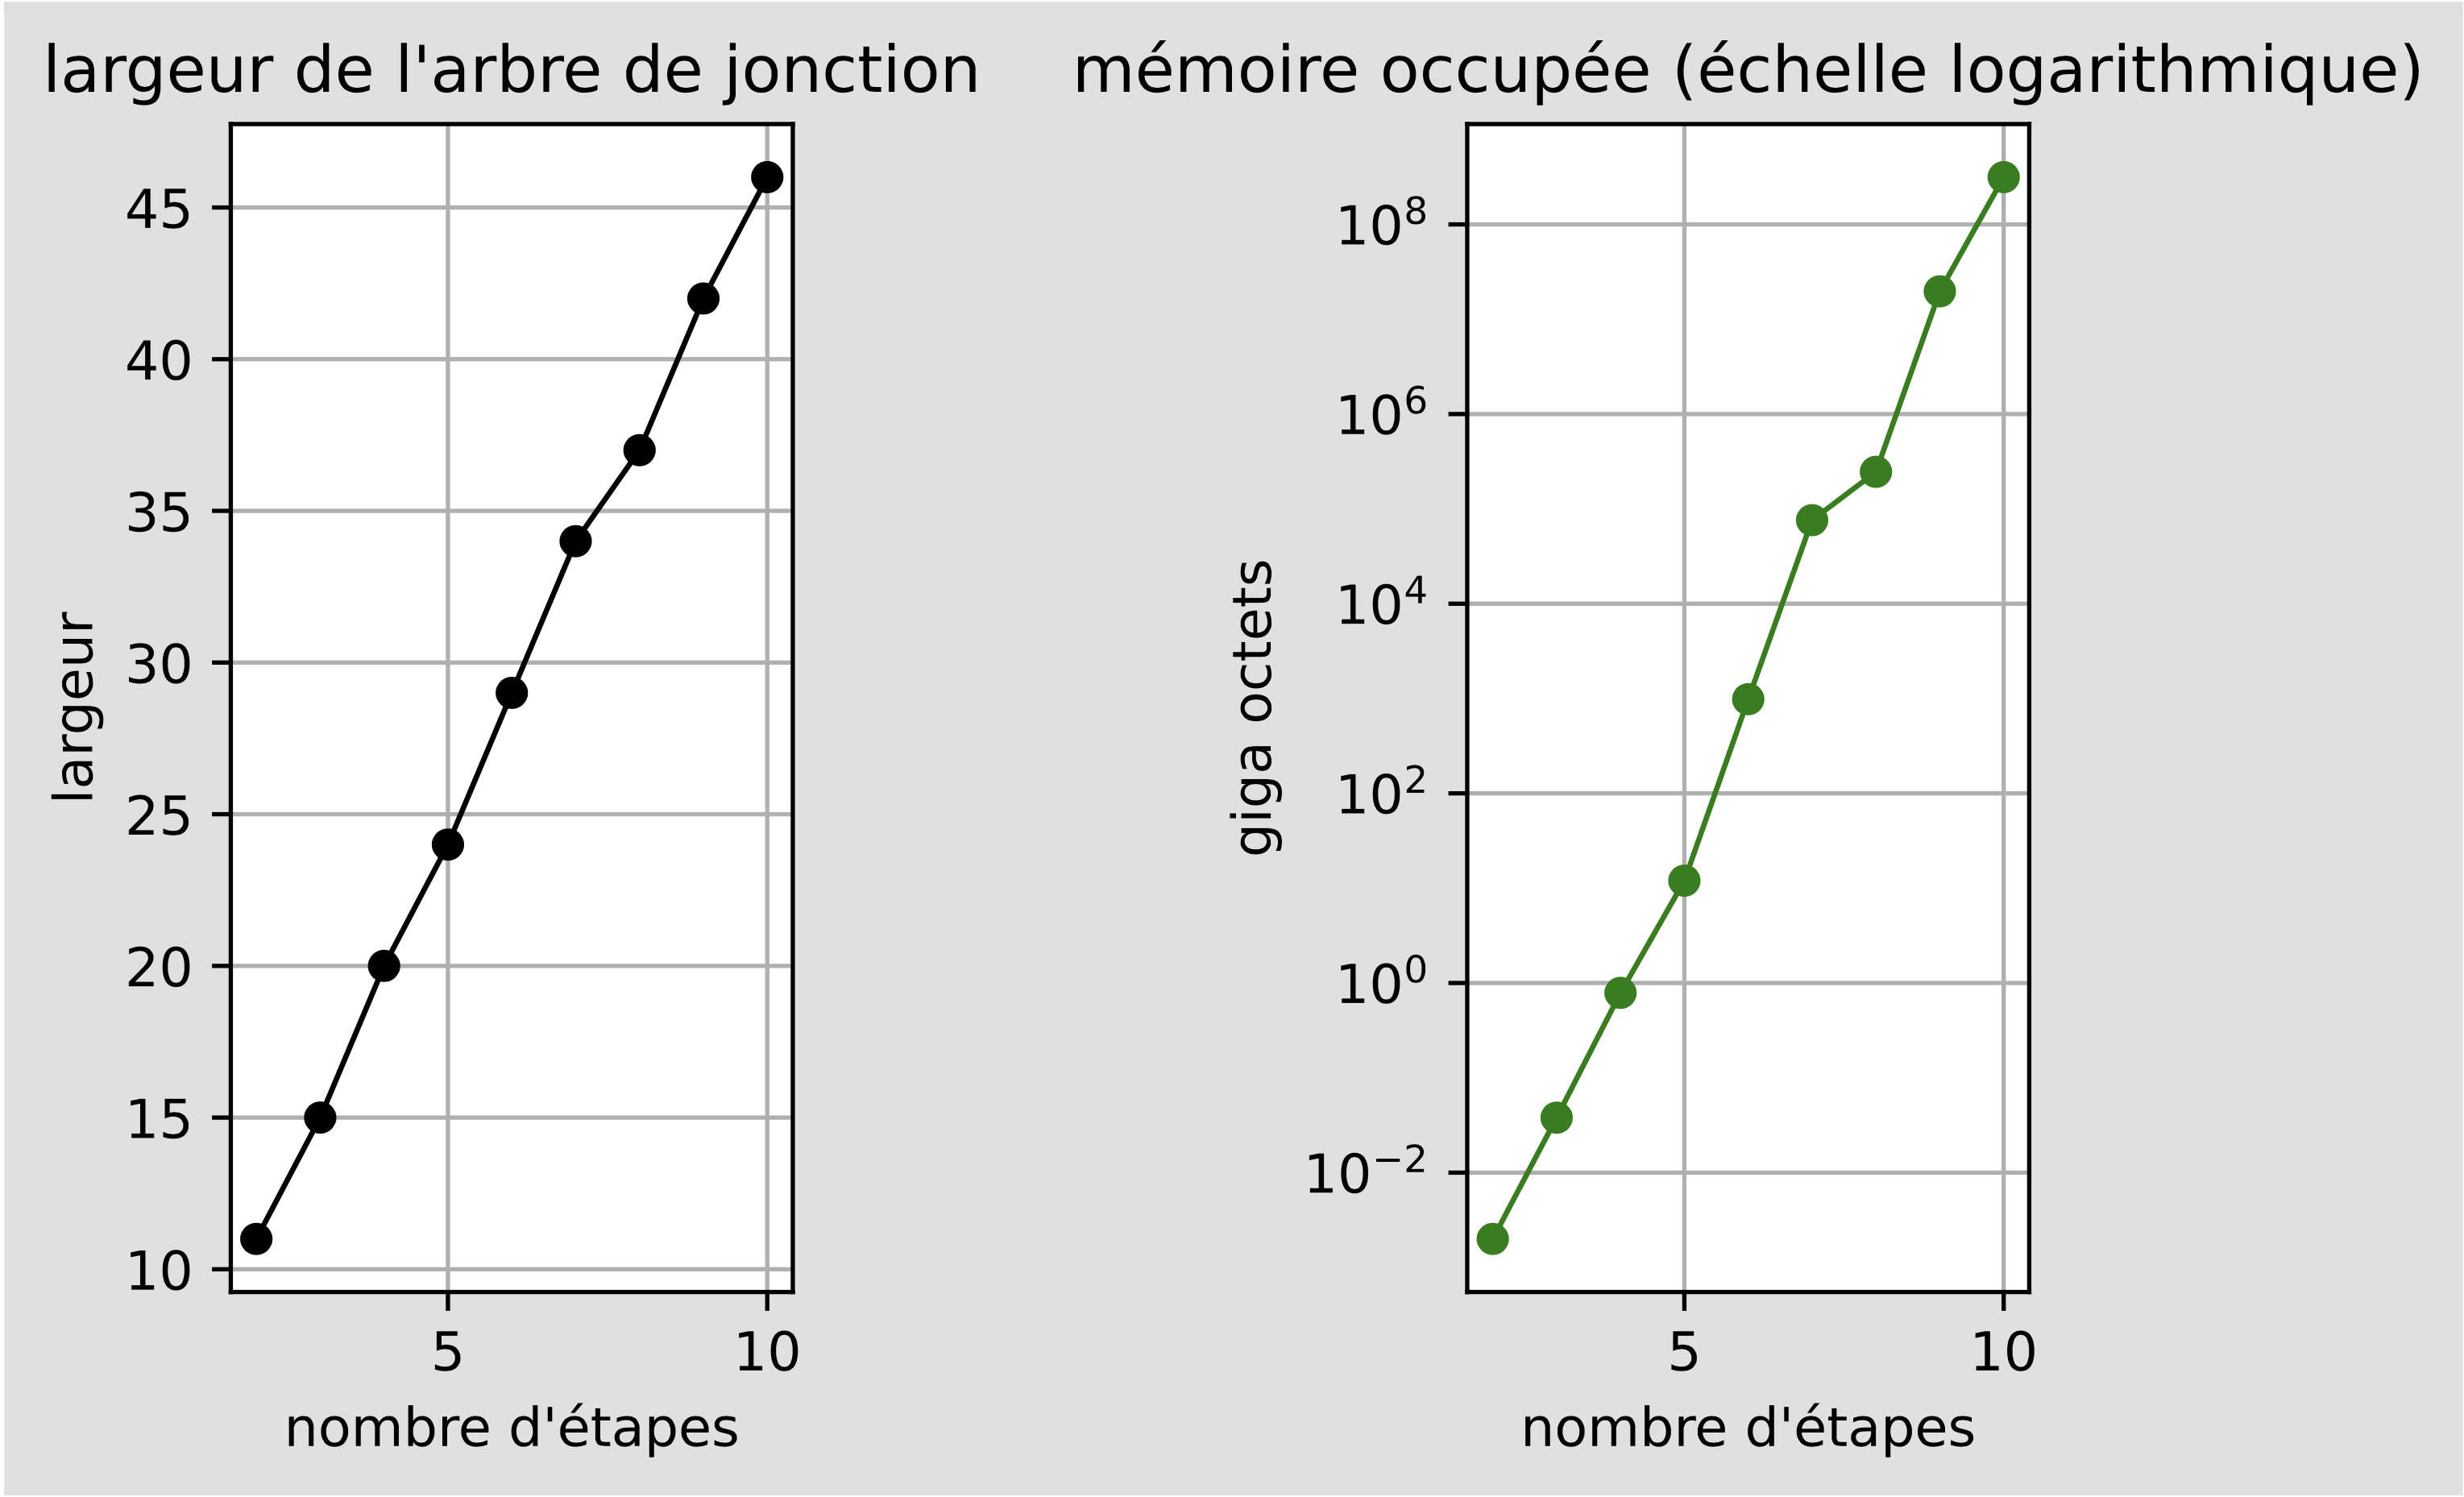
\includegraphics[scale=0.2]{docs/ressources_rapport/graphes.png}
\caption{Graphes sur la complexité en temps et espace des méthodes actuelles}
\end{figure}

On parvient à résoudre cet ID avec les méthodes exactes actuelles (une machine avec 128Go de mémoire vive) sur des instances du problèmes comprenant jusqu'à 5 étapes. Au delà de 5 étapes, la mémoire nécessaire et le temps pour trouver la solution explose. \bigbreak
Il n'est pas envisageable de concevoir une machine capable de stocker autant de données pour résoudre de façon exacte cet ID. Il y a donc un réel besoin d'avoir une implémentation permettant de résoudre plus rapidement les IDs et en nécessitant moins d'espace.
\bigbreak
\bigbreak

\subsection{But du projet}
Le but de ce projet est donc d'étudier un algorithme de Branch and Bound pour résoudre des LIMIDs dans un petit graphe de recherche dans lequel différents chemins menant au même nœud représentent différentes histoires. Pour résoudre ce type de problème à grande complexité en espace et en temps, on doit tirer parti des opportunités pour le calcul de stratégie, utiliser des techniques d'inférence probabiliste et calculer les limites dans un graphe.
Enfin, il est envisagé l'intégrer l'algorithme dans la librairie Python PyAgrum.

\section{Explication de l'algorithme de Branch and Bound}
Les LIMIDs sont résolus en trouvant une stratégie qui maximise l'utilité prévue.
L'algorithme étudié dans ce projet résout les LIMIDs en les convertissant en un graphe ET/OU puis en effectuant un parcours en profondeur sur ces derniers.
Les nœuds ET sont alors des variables aléatoires correspondant aux nœuds chances qui sont informatifs à un nœud de décision et les nœuds OU sont des nœuds de décision (représentant des alternatives de décision), enfin les feuilles sont les nœuds d'utilités.
Un chemin racine-feuille représente alors une instance des nœuds d'information et de décision.
En effectuant un parcours en profondeur d'abord, on peut générer l'arbre à la volée et ne garder qu'une partie de l'arborescence en mémoire.
Deux problèmes se posent alors, le calcul des limites et celui des probabilités postérieures.

\section{Déliverables du projet}
Le projet a pour but de réaliser :
\begin{itemize}
\item Un état de l'art et stabilisation des algorithmes pour la résolution avec Branch and Bound, en particulier l'analyse du calcul des bornes et des probabilités postérieures.
\item Une implémentation efficace et compacte des arbres ET/OU.
\item Une intégration de l'algorithme correctement documentée (style python en anglais) dans l'API pyAgrum vérifiant l'implémentation des méthodes (liste non exhaustive) :
\begin{itemize}
    \item makeInference : Réalise l'inférence sur un LIMID.
    \item PosterieurUtility : Retourne la probabilité postérieure d'un noeud.
    \item lIMInfluenceDiagram : Retourne le LIMID associé à l'instance de la classe.
    \item optimalDecision : Retourne la décision optimale pour un certain noeud décision basé sur le critère MEU.
    \item MEU : Retourne l'utilité maximate espérée de l'inférence.
    \item junctionTree : Retourne l'arbre de jonction associé au LIMID
    \item andOrTree: Retourne le graphe de jonction développé
    \item une fonction pour avoir le graphe/arbre du branch and bound + une fonction pour avoir les états?
\end{itemize}
\item Une série de tests unitaires effectués sur les méthodes avec l'API TestUnit.
\item Une série de benchmark validant l'utilité de notre implémentation de la méthode branch and bound face aux méthodes existante.
\end{itemize}


 %il y a un repertoire dans pyagrum sur les tests ou on va rajouter les tests (on utilise UnitTest)
 
 %lien pour les codes de test dans pyagrul : https://gitlab.com/agrumery/aGrUM/-/blob/master/wrappers/pyAgrum/testunits/tests/AggregatorsForBNTestSuite.py
 
 %lien pour voir la documentation : https://gitlab.com/agrumery/aGrUM/-/blob/master/wrappers/pyAgrum/pyLibs/causal/_CausalFormula.py

%\section{Implémentation de l'algorithme dans pyAgrum}




\end{document}